\label{Jena}

Im folgenden soll skizziert werden, wie die Webseite des Online-Assessment-Tests bereitgestellt und präsentiert wird.
Dazu wird zunächst ein Überblick über die durch den Generator bereitgestellten statischen Dateien erstellt. Anschließend wird beschrieben, wie aus den statischen Daten die Seiten der Webseite zusammengestellt werden.
Ein besonderer Schwerpunkt liegt dabei auf der Anzeige der Fragen und der damit verbundenen Verwaltung des Zustandes.
Zuletzt wird die Auswertung und die Anzeige der Evaluierung des Tests beleuchtet.

\subsubsection{Überblick über die statischen Dateien}

Die im Abschnitt zuvor erwähnten statischen Dateien im durch den Generator erzeugten Zip-Archiv bestehen aus:

\begin{itemize}
\item einer einzelnen HTML-Seite, welche rudimentär mit zu ersetzenden Elementen gefüllt ist

\item den CSS-Dateien für das Styling der Seiten

\item den JavaScript-Dateien zur Manipulation der HTML-Seite 

\item den Fragen in Form von HTML und JSON-Dateien

\item und die im Text verwendeten Bilder und Videos
\end{itemize}

Die genannten Dateien werden anschließend mithilfe eines HTTP-Servers dem Client angeboten. 

\subsubsection{Anzeige der Fragen}

Die gesamte Webseite basiert auf einer einzelnen HTML-Seite, die für jede Frage des Tests verändert wird.
Ist im folgenden die Rede von einer Seite, so wird damit entsprechend die manipulierte HTML-Seite für eine Frage referenziert.

 \begin{figure*} 
  \centering
     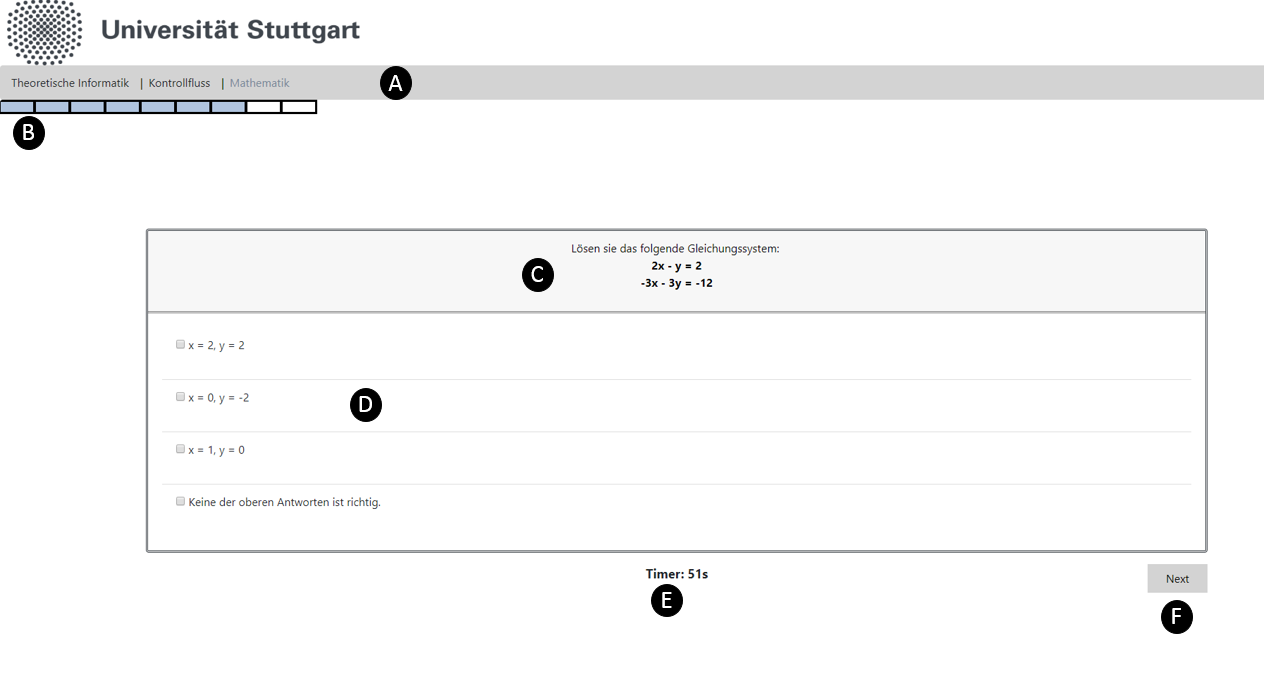
\includegraphics[width=\textwidth]{Jena_Images/beispielfrage.png}
  \caption{Die Anzeige einer Frage für einen Beispieltest.}
  \label{fig:beispielfrage}
\end{figure*}
Im folgenden soll der Aufbau jeder Fragenseite, zu sehen in Abbildung~\ref{fig:beispielfrage}, von oben nach unten betrachtet und erläutert werden. 
  
Die Seiten beginnen stets mit dem Logo der Universität Stuttgart. 
Es folgt eine Übersichtsleiste (A), welche die verschiedenen Kategorien des Tests anzeigt. 
Die Kategorie der aktuell angezeigten Frage wird zur Hervorhebung grau markiert. 

Unterhalb der Übersichtsleiste findet sich der Fortschrittsbalken (B). 
Dieser setzt sich aus $n$ kleineren Balken zusammen, wobei $n$ die Gesamtanzahl aller Fragen ist.
Die Anzahl der gefüllten Balken gibt dabei an, wie viele Fragen, inklusive der aktuellen Frage, bisher beantwortet wurden, die Anzahl der leeren Balken stellt dagegen die verbleibende Anzahl an Frage dar. 

Unterhalb des Fortschrittsbalkens und zentral im Sichtfeld werden die aktuelle Frage und ihre Antwortmöglichkeiten angezeigt. 
Die Frage erhält ein eigenes Feld (C), in welcher optional eine Erklärung zur Frage und ein Bild angezeigt werden können.
Separiert von der Frage folgen dann ihre Antwortmöglichkeiten (D), die jeweils eigene Felder erhalten. 
Für alle Fragen wird links neben jeder Antwort eine Checkbox platziert.
Hierbei können Antworten auch Bilder beinhalten, die innerhalb der Antwortfelder angezeigt werden.
Wurde die optionale Zeitbeschränkung für die Frage aktiviert, so wird die verbleibende Zeit (E) mittig und unterhalb dem Feld der Frage und ihrer Antworten angezeigt.

Zuletzt findet sich der Next-Button (F) rechtsbündig unter dem Feld der Frage und ihrer Antworten, mit welchem die nächste Frage anzeigen lässt.

Es wird zunächst die nahezu leere HTML-Seite aufgerufen, welche als Hülle für die Seiten der Fragen dient. 
In der Folge wird der Inhalt der HMTL-Seite durch die aktuell anzuzeigende Frage bestimmt.

Für jede Frage des Online-Assessment-Tests wird das Codefragment, welches zur Anzeige der Frage benötigt wird, aus der serverseitig gespeicherten HTML-Datei der Frage gelesen und in das HTML-Dokument geschrieben. 
Zusätzlich legt eine JSON-Datei pro Frage das optionale Zeitlimit und die Punkte für die korrekte Beantwortung der Frage fest.

Die bisher angezeigten und beantworteten Fragen werden im Rahmen der Zustandsverwaltung mitverwaltet, die aktuelle Frage wird dann anhand des Zustands abgeleitet.

\subsubsection{Zustandsverwaltung}

Der Zustand der Webseite setzt sich im wesentlichen aus den bisher beantworteten Fragen und ihren Antwortmöglichkeiten zusammen. 
Für jede beantwortete Frage wird ein Bitstring der Länge $m$ verwaltet. Dieser gibt an, wie viele Antwortmöglichkeiten die Frage aufweißt und wie die Frage durch den Nutzer beantwortet wurde. 
Die Anzahl der Antwortmöglichkeiten einer Frage wird in den ersten $5$ Bit des Bitstrings kodiert. 
Die restlichen $m - 5$ Bit des Bitstrings stellen die einzelnen Antwortmöglichkeiten der Frage dar. Jede einzelne Antwortmöglichkeit wird dabei durch ein einzelnes Bit repräsentiert, welches genau dann gesetzt ist, wenn die Antwortmöglichkeit angekreuzt wurde.
Wird beispielsweise eine Frage mit $3$ Antwortmöglichkeiten gestellt, wobei nur die erste der drei Antwortmöglichkeiten angekreuzt wurde, so ist der resultierende Bitstring der Länge $8$ für diese Frage $00011100$.

Die einzelnen Bitstrings der jeweiligen Fragen werden dann konkateniert und der resultierende String durch die Umwandlung in \textit{Base64} verkürzt. 
Anschließend wird diese Zeichenfolge als URL-Parameter an die aktuelle URL angehängt.
 
Für die Anzeige einer Frage wird somit die aktuelle URL abgerufen, der URL-Parameter extrahiert und dekodiert.
Aus dem dekodierten Bitstring wird dann die Anzahl bisher beantworteter Fragen errechnet und anhand dessen die HTML und JSON-Datei der aktuellen Frage abgeleitet.

Beim initialen Aufruf der Webseite wird somit die erste Frage angezeigt, wobei der URL-Parameter leer ist.
Beim Drücken des Next-Buttons werden dann die Antworten ausgewertet, ehe das Skript zur Verwaltung des Zustandes mit dem Ergebnis aufgerufen wird. 
Die URL wird dann entsprechend angepasst und die nächste Frage geladen.

\subsubsection{Evaluierung}

Wurde die letzte Frage erreicht und der Next-Button gedrückt, wird der finale Zustand aus der URL gelesen.
Anschließend wird das Skript zur Auswertung der Evaluation aufgerufen. 
Dieses Skript vergleicht die Antworten des Nutzers mit einem durch den Generator bereitgestellten Lösungsstring.
Für jede korrekt beantwortete Frage wird die durch die Frage vergebene Punktzahl zur erreichten Kategoriepunktzahl und Gesamtpunktzahl addiert.
Die Kategoriepunktzahl gibt die erreichte Punktzahl für sämtliche Fragen einer Kategorie an, die Gesamtpunktzahl die erreichte Punktzahl für die Gesamtheit aller Fragen.

 \begin{figure*} 
  \centering
     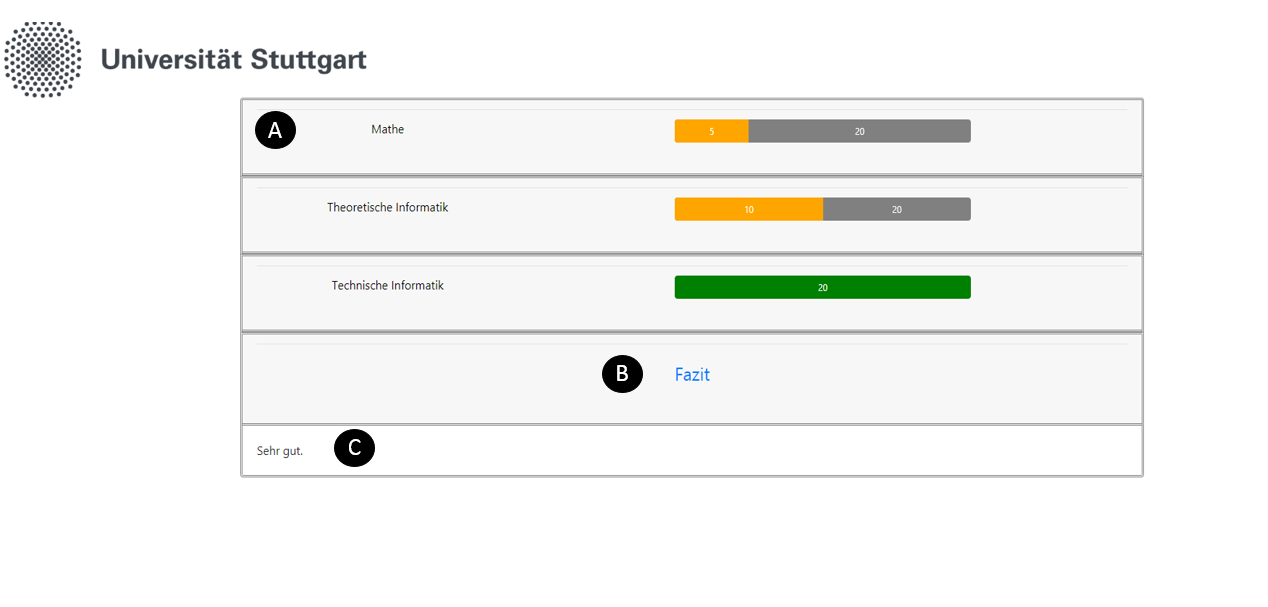
\includegraphics[width=\textwidth]{Jena_Images/eval.png}
  \caption{Die Evaluationsseite für einen Beispieltest mit drei Kategorien und maximal erreichbaren 60 Punkten.}
  \label{fig:eval}
\end{figure*}
Die verschiedenen Kategoriepunktzahlen und die Gesamtpunktzahl werden dann in einer spezifischen Evaluationsseite dargestellt, die in Abbildung~\ref{fig:eval} zu sehen ist.
  
Die Evaluationsseite setzt sich aus der Anzeige der erreichten Punkte für jede einzelne Kategorie (A) und einem Fazit abhängig von der Gesamtpunktzahl (B) zusammen.
Für die einzelnen Kategorien wird anhand eines Fortschrittsbalkens angezeigt, wie viele der maximal erreichbaren Punkte der betroffenen Kategorie erreicht wurden. 

Für das Fazit wird eine spezifische JSON-Datei anhand der erreichten Gesamtpunktzahl ausgewertet. 
Der Ersteller des Tests legt in dieser Datei fest, welcher Fazittext für welches Punkteintervall angezeigt werden soll. 
Es wird dann überpürft in welchem Intervall die erreichte Gesamtpunktzahl liegt und das entsprechende Fazit im Dropdown-Feld unter den Fortschrittsbalken angezeigt (C). 
